\section{Performance Benchmark and Overlay Scalability}

\subsection{Benchmark Objective}
Mục tiêu của benchmark là trả lời câu hỏi:

\begin{quote}
Full mesh broadcast và DHT-based broadcast khác nhau thế nào khi số peer tăng?
\end{quote}

Benchmark này \textbf{không} nhằm chứng minh một mode luôn tốt hơn mode còn lại. Thay vào đó, nó đánh giá trade-off giữa \textit{direct delivery latency} và \textit{connection scalability}:
\begin{quote}
This benchmark does not aim to prove that one mode is always better. Instead, it evaluates the trade-off between direct delivery latency and connection scalability.
\end{quote}

\subsection{Benchmark Setup}
Setup thực nghiệm:
\begin{itemize}[leftmargin=2em]
    \item Each peer is executed as a separate Python process.
    \item A tracker process is used for discovery and membership.
    \item Both modes run on the same machine.
    \item Authentication is disabled or bypassed for benchmark purpose if applicable.
    \item The benchmark records JSON and Markdown logs after each run.
\end{itemize}

Các biến đầu vào trong ma trận benchmark:
\begin{itemize}[leftmargin=2em]
    \item \texttt{nodes}: 10, 20, \ldots, 100
    \item \texttt{messages}: 20
    \item \texttt{payload}: 256 bytes
\end{itemize}

Các metric chính được ghi nhận:
\begin{itemize}[leftmargin=2em]
    \item total peer connections
    \item delivery success rate
    \item duplicate count
    \item p50 latency
    \item p95 latency
    \item max latency
    \item RSS memory
\end{itemize}

\subsection{Connection Scalability}
Full mesh yêu cầu mỗi peer kết nối trực tiếp đến mọi peer còn lại, do đó số lượng kết nối trực tiếp tăng theo bậc hai khi số node tăng. Ngược lại, DHT overlay duy trì một tập kết nối overlay nhỏ hơn, và chuyển tiếp bản tin qua lớp overlay thay vì fan-out trực tiếp đến toàn bộ members.

\begin{figure}[H]
\centering
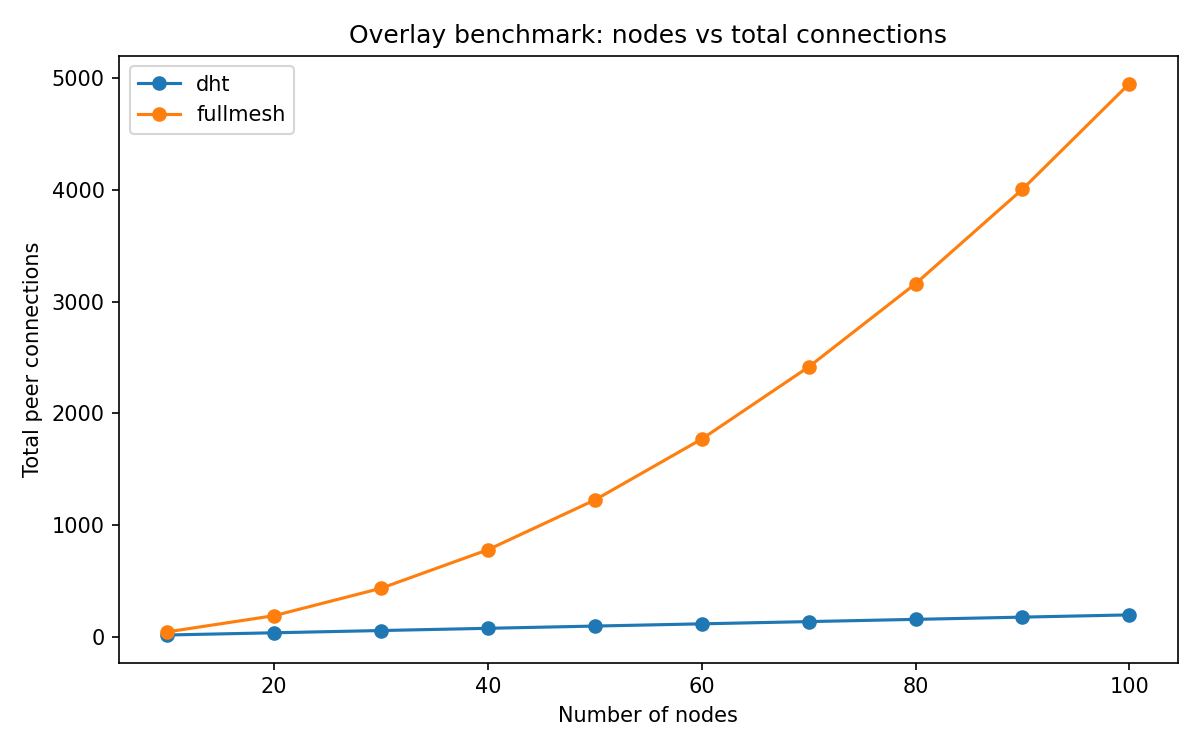
\includegraphics[width=\textwidth]{assets/benchmark-plots/nodes_vs_connections.png}
\caption{Total peer connections as the number of nodes increases. Full mesh grows quadratically, while the DHT overlay keeps the direct connection count significantly lower.}
\end{figure}

\subsection{Latency Trade-off}
Ở quy mô nhỏ, full mesh thường có p95 latency thấp hơn vì đường truyền là direct delivery. Khi số node tăng, số lượng kết nối và overhead quản lý socket của full mesh tăng mạnh, và DHT trở nên cạnh tranh (hoặc tốt hơn) về tail latency trong một số cấu hình.

\begin{figure}[H]
\centering
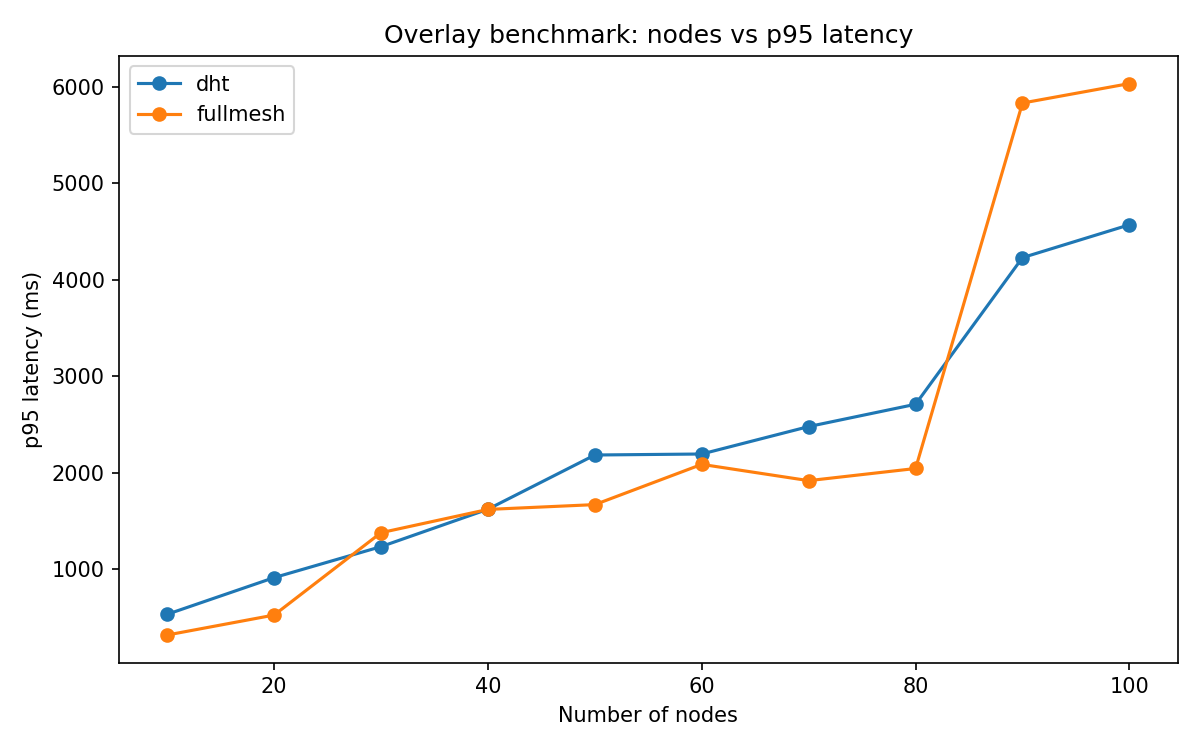
\includegraphics[width=\textwidth]{assets/benchmark-plots/nodes_vs_p95_latency.png}
\caption{Tail latency (p95) as the number of nodes increases. Full mesh benefits from direct delivery at small scale, while the DHT overlay trades routing hops for better connection scalability.}
\end{figure}

\subsection{Reliability and Delivery Correctness}
Các benchmark run đã hoàn tất cho thấy cả hai overlay đều đạt delivery correctness tốt. Trong các run đã hoàn thành, hai overlay đều giao đủ số message kỳ vọng với \textbf{zero failures} và \textbf{zero duplicates}. Kết quả này bổ sung cho Section 07: phần failure handling tập trung vào xử lý lỗi ở mức protocol/runtime, còn benchmark ở đây kiểm chứng rằng cơ chế broadcast không tạo duplicate hoặc làm mất message trong điều kiện test.

\begin{figure}[H]
\centering
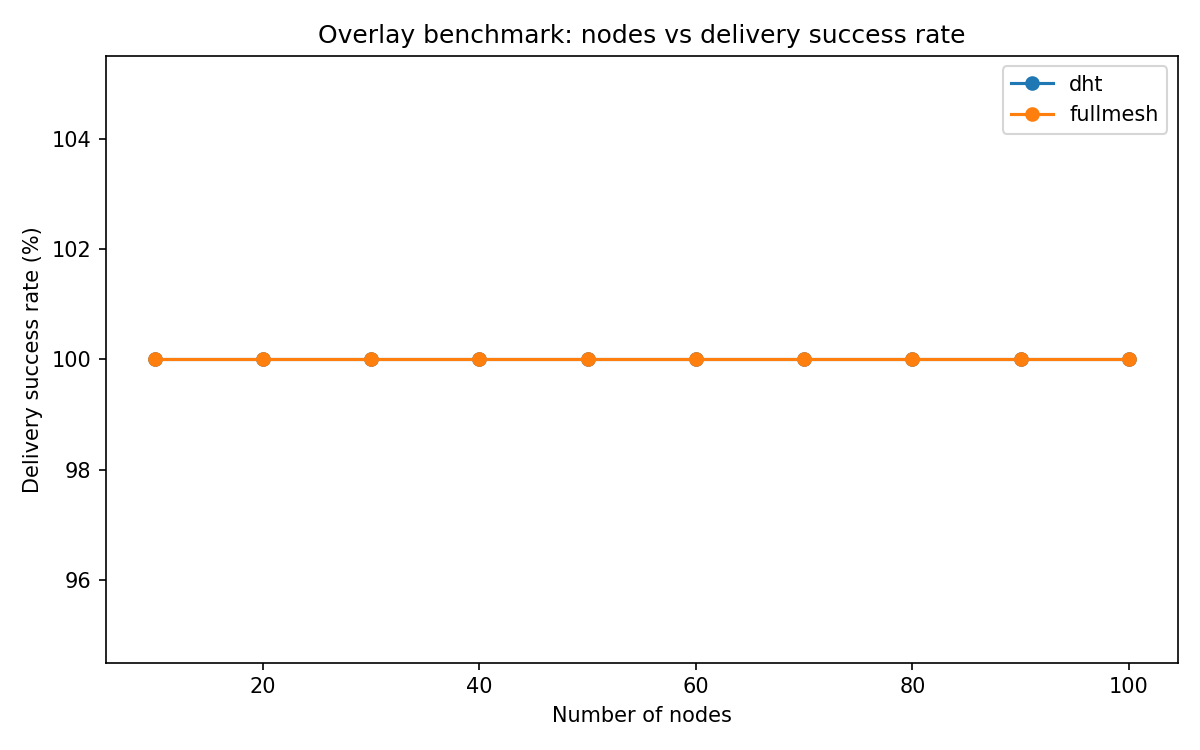
\includegraphics[width=\textwidth]{assets/benchmark-plots/nodes_vs_success_rate.png}
\caption{Delivery success rate as the number of nodes increases. Completed runs show no missing deliveries and no duplicates.}
\end{figure}

\subsection{Memory Observation}
RSS memory quan sát được khá tương đồng giữa hai mode vì benchmark khởi tạo một Python process cho mỗi peer. Do đó, memory chủ yếu bị chi phối bởi overhead runtime theo process, không chỉ bởi số lượng socket/kết nối.

\begin{figure}[H]
\centering
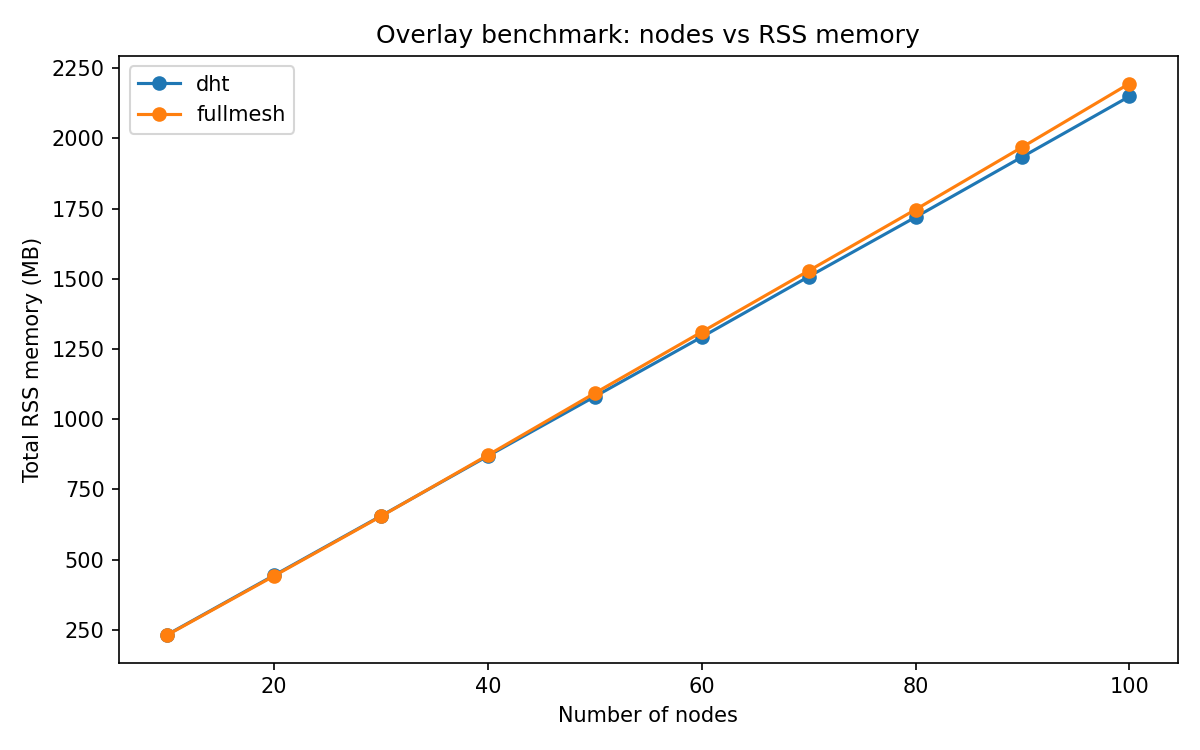
\includegraphics[width=\textwidth]{assets/benchmark-plots/nodes_vs_rss_mb_total.png}
\caption{Total RSS memory versus node count. Memory is largely dominated by per-process runtime overhead in this benchmark setup.}
\end{figure}

\subsection{Summary}
Tóm lại:
\begin{itemize}[leftmargin=2em]
    \item Full mesh đơn giản và latency-efficient ở quy mô nhỏ, nhưng số lượng kết nối tăng rất nhanh khi số node tăng.
    \item DHT thêm routing overhead (forwarding qua overlay), nhưng giảm mạnh số kết nối trực tiếp và phù hợp hơn khi cần mở rộng số peer.
\end{itemize}
